\documentclass[twoside]{book}

% Packages required by doxygen
\usepackage{fixltx2e}
\usepackage{calc}
\usepackage{doxygen}
\usepackage[export]{adjustbox} % also loads graphicx
\usepackage{graphicx}
\usepackage[utf8]{inputenc}
\usepackage{makeidx}
\usepackage{multicol}
\usepackage{multirow}
\PassOptionsToPackage{warn}{textcomp}
\usepackage{textcomp}
\usepackage[nointegrals]{wasysym}
\usepackage[table]{xcolor}

% Font selection
\usepackage[T1]{fontenc}
\usepackage[scaled=.90]{helvet}
\usepackage{courier}
\usepackage{amssymb}
\usepackage{sectsty}
\renewcommand{\familydefault}{\sfdefault}
\allsectionsfont{%
  \fontseries{bc}\selectfont%
  \color{darkgray}%
}
\renewcommand{\DoxyLabelFont}{%
  \fontseries{bc}\selectfont%
  \color{darkgray}%
}
\newcommand{\+}{\discretionary{\mbox{\scriptsize$\hookleftarrow$}}{}{}}

% Page & text layout
\usepackage{geometry}
\geometry{%
  a4paper,%
  top=2.5cm,%
  bottom=2.5cm,%
  left=2.5cm,%
  right=2.5cm%
}
\tolerance=750
\hfuzz=15pt
\hbadness=750
\setlength{\emergencystretch}{15pt}
\setlength{\parindent}{0cm}
\setlength{\parskip}{3ex plus 2ex minus 2ex}
\makeatletter
\renewcommand{\paragraph}{%
  \@startsection{paragraph}{4}{0ex}{-1.0ex}{1.0ex}{%
    \normalfont\normalsize\bfseries\SS@parafont%
  }%
}
\renewcommand{\subparagraph}{%
  \@startsection{subparagraph}{5}{0ex}{-1.0ex}{1.0ex}{%
    \normalfont\normalsize\bfseries\SS@subparafont%
  }%
}
\makeatother

% Headers & footers
\usepackage{fancyhdr}
\pagestyle{fancyplain}
\fancyhead[LE]{\fancyplain{}{\bfseries\thepage}}
\fancyhead[CE]{\fancyplain{}{}}
\fancyhead[RE]{\fancyplain{}{\bfseries\leftmark}}
\fancyhead[LO]{\fancyplain{}{\bfseries\rightmark}}
\fancyhead[CO]{\fancyplain{}{}}
\fancyhead[RO]{\fancyplain{}{\bfseries\thepage}}
\fancyfoot[LE]{\fancyplain{}{}}
\fancyfoot[CE]{\fancyplain{}{}}
\fancyfoot[RE]{\fancyplain{}{\bfseries\scriptsize Generated by Doxygen }}
\fancyfoot[LO]{\fancyplain{}{\bfseries\scriptsize Generated by Doxygen }}
\fancyfoot[CO]{\fancyplain{}{}}
\fancyfoot[RO]{\fancyplain{}{}}
\renewcommand{\footrulewidth}{0.4pt}
\renewcommand{\chaptermark}[1]{%
  \markboth{#1}{}%
}
\renewcommand{\sectionmark}[1]{%
  \markright{\thesection\ #1}%
}

% Indices & bibliography
\usepackage{natbib}
\usepackage[titles]{tocloft}
\setcounter{tocdepth}{3}
\setcounter{secnumdepth}{5}
\makeindex

% Hyperlinks (required, but should be loaded last)
\usepackage{ifpdf}
\ifpdf
  \usepackage[pdftex,pagebackref=true]{hyperref}
\else
  \usepackage[ps2pdf,pagebackref=true]{hyperref}
\fi
\hypersetup{%
  colorlinks=true,%
  linkcolor=blue,%
  citecolor=blue,%
  unicode%
}

% Custom commands
\newcommand{\clearemptydoublepage}{%
  \newpage{\pagestyle{empty}\cleardoublepage}%
}

\usepackage{caption}
\captionsetup{labelsep=space,justification=centering,font={bf},singlelinecheck=off,skip=4pt,position=top}

%===== C O N T E N T S =====

\begin{document}

% Titlepage & ToC
\hypersetup{pageanchor=false,
             bookmarksnumbered=true,
             pdfencoding=unicode
            }
\pagenumbering{alph}
\begin{titlepage}
\vspace*{7cm}
\begin{center}%
{\Large Eco\+Net Documentation }\\
\vspace*{1cm}
{\large Generated by Doxygen 1.8.14}\\
\end{center}
\end{titlepage}
\clearemptydoublepage
\pagenumbering{roman}
\tableofcontents
\clearemptydoublepage
\pagenumbering{arabic}
\hypersetup{pageanchor=true}

%--- Begin generated contents ---
\chapter{Class Index}
\section{Class List}
Here are the classes, structs, unions and interfaces with brief descriptions\+:\begin{DoxyCompactList}
\item\contentsline{section}{\mbox{\hyperlink{class_abilities_editor}{Abilities\+Editor}} \\*A\+PI for Abilities objects. Modifies tentative\+Abilities variable from \mbox{\hyperlink{class_creature_editor}{Creature\+Editor}} }{\pageref{class_abilities_editor}}{}
\item\contentsline{section}{\mbox{\hyperlink{class_ability}{Ability}} \\*Modifies creature\textquotesingle{}s ability to consume certain resources or attack certain species. Each creature has a specific number of ability points to assign to different abilities. }{\pageref{class_ability}}{}
\item\contentsline{section}{\mbox{\hyperlink{class_action}{Action}} }{\pageref{class_action}}{}
\item\contentsline{section}{\mbox{\hyperlink{class_action_editor}{Action\+Editor}} }{\pageref{class_action_editor}}{}
\item\contentsline{section}{\mbox{\hyperlink{class_action_editor_abstract}{Action\+Editor\+Abstract}} }{\pageref{class_action_editor_abstract}}{}
\item\contentsline{section}{\mbox{\hyperlink{interface_activation_behavior}{Activation\+Behavior}} \\*Interface for objects that implement an activation function. }{\pageref{interface_activation_behavior}}{}
\item\contentsline{section}{\mbox{\hyperlink{class_bias_node}{Bias\+Node}} }{\pageref{class_bias_node}}{}
\item\contentsline{section}{\mbox{\hyperlink{class_boost_requirement}{Boost\+Requirement}} \\*Currently not used. Boost requirements allow for modifications to abilities, thus giving creatures with certain resources an advantage over other creatures. If all creatures are capable of this ability, and have the same boost requirements, they all have the opportunity to gain this advantage. However, it should be noted that the relationship between resources and abilities established here does give certain resources more inherent value than others. }{\pageref{class_boost_requirement}}{}
\item\contentsline{section}{\mbox{\hyperlink{class_camera_positioner}{Camera\+Positioner}} }{\pageref{class_camera_positioner}}{}
\item\contentsline{section}{\mbox{\hyperlink{class_comm_action}{Comm\+Action}} }{\pageref{class_comm_action}}{}
\item\contentsline{section}{\mbox{\hyperlink{class_comm_action_editor}{Comm\+Action\+Editor}} }{\pageref{class_comm_action_editor}}{}
\item\contentsline{section}{\mbox{\hyperlink{class_comm_input_node}{Comm\+Input\+Node}} }{\pageref{class_comm_input_node}}{}
\item\contentsline{section}{\mbox{\hyperlink{class_comm_network}{Comm\+Network}} \\*A network that converts incomming comm signals into action recommendations. A seperate comm network is needed for every neightbor that sends a comm signal. }{\pageref{class_comm_network}}{}
\item\contentsline{section}{\mbox{\hyperlink{class_comm_node_editor}{Comm\+Node\+Editor}} \\*A\+PI for Comm Nodes }{\pageref{class_comm_node_editor}}{}
\item\contentsline{section}{\mbox{\hyperlink{class_comm_signal}{Comm\+Signal}} \\*The comm network must individually process each comm signal stored in the creatures comm\+List, and save the outputs as action recommendations. }{\pageref{class_comm_signal}}{}
\item\contentsline{section}{\mbox{\hyperlink{class_consume_from_land}{Consume\+From\+Land}} }{\pageref{class_consume_from_land}}{}
\item\contentsline{section}{\mbox{\hyperlink{class_consume_from_land_editor}{Consume\+From\+Land\+Editor}} }{\pageref{class_consume_from_land_editor}}{}
\item\contentsline{section}{\mbox{\hyperlink{class_copier}{Copier}} }{\pageref{class_copier}}{}
\item\contentsline{section}{\mbox{\hyperlink{class_creat_menu_behav}{Creat\+Menu\+Behav}} }{\pageref{class_creat_menu_behav}}{}
\item\contentsline{section}{\mbox{\hyperlink{class_creature}{Creature}} \\*Class for storing all data about a creature/agent, including its neural networks, queued actions, stored resources, location and other parameters. }{\pageref{class_creature}}{}
\item\contentsline{section}{\mbox{\hyperlink{class_creature_editor}{Creature\+Editor}} }{\pageref{class_creature_editor}}{}
\item\contentsline{section}{\mbox{\hyperlink{class_creature_resource}{Creature\+Resource}} \\*Resource stored by a creature, and how that resource effects the creature. }{\pageref{class_creature_resource}}{}
\item\contentsline{section}{\mbox{\hyperlink{class_eco_manager}{Eco\+Manager}} }{\pageref{class_eco_manager}}{}
\item\contentsline{section}{\mbox{\hyperlink{class_eco_menu_behav}{Eco\+Menu\+Behav}} }{\pageref{class_eco_menu_behav}}{}
\item\contentsline{section}{\mbox{\hyperlink{class_eco_menu_tester}{Eco\+Menu\+Tester}} }{\pageref{class_eco_menu_tester}}{}
\item\contentsline{section}{\mbox{\hyperlink{class_ecosystem}{Ecosystem}} \\*This class contains all of the data about the state of the ecosystem including the populations, species templates, map, resources, and other general parameters. }{\pageref{class_ecosystem}}{}
\item\contentsline{section}{\mbox{\hyperlink{class_ecosystem_editor}{Ecosystem\+Editor}} \\*A\+PI for alterning ecosystem. }{\pageref{class_ecosystem_editor}}{}
\item\contentsline{section}{\mbox{\hyperlink{class_ecosystem_getter}{Ecosystem\+Getter}} }{\pageref{class_ecosystem_getter}}{}
\item\contentsline{section}{\mbox{\hyperlink{class_empty_activ_behavior}{Empty\+Activ\+Behavior}} \\*No activation function (node simply uses linear combination). }{\pageref{class_empty_activ_behavior}}{}
\item\contentsline{section}{\mbox{\hyperlink{class_error_manager}{Error\+Manager}} }{\pageref{class_error_manager}}{}
\item\contentsline{section}{\mbox{\hyperlink{class_game_manager}{Game\+Manager}} }{\pageref{class_game_manager}}{}
\item\contentsline{section}{\mbox{\hyperlink{class_helper_validator}{Helper\+Validator}} }{\pageref{class_helper_validator}}{}
\item\contentsline{section}{\mbox{\hyperlink{interface_i_ecosystem_editor}{I\+Ecosystem\+Editor}} }{\pageref{interface_i_ecosystem_editor}}{}
\item\contentsline{section}{\mbox{\hyperlink{class_inner_input_node}{Inner\+Input\+Node}} }{\pageref{class_inner_input_node}}{}
\item\contentsline{section}{\mbox{\hyperlink{class_inner_input_node_editor}{Inner\+Input\+Node\+Editor}} \\*A\+PI for Inner\+Input\+Nodes. }{\pageref{class_inner_input_node_editor}}{}
\item\contentsline{section}{\mbox{\hyperlink{class_land}{Land}} \\*Class for storing data about a location on the map. Also facilitates creature\textquotesingle{}s interaction with the environment. }{\pageref{class_land}}{}
\item\contentsline{section}{\mbox{\hyperlink{class_land_resource_editor}{Land\+Resource\+Editor}} \\*Used as interface for generating \mbox{\hyperlink{class_resource_store}{Resource\+Store}} objects. }{\pageref{class_land_resource_editor}}{}
\item\contentsline{section}{\mbox{\hyperlink{class_logistic_activ_behavior}{Logistic\+Activ\+Behavior}} \\*Implements logistic activation function. }{\pageref{class_logistic_activ_behavior}}{}
\item\contentsline{section}{\mbox{\hyperlink{class_logistic_with_neg_activ_behav}{Logistic\+With\+Neg\+Activ\+Behav}} \\*Logistic activation function, but mapped to \mbox{[}-\/1,1\mbox{]} }{\pageref{class_logistic_with_neg_activ_behav}}{}
\item\contentsline{section}{\mbox{\hyperlink{class_l_r_menu_behav}{L\+R\+Menu\+Behav}} }{\pageref{class_l_r_menu_behav}}{}
\item\contentsline{section}{\mbox{\hyperlink{class_main_menu_behav}{Main\+Menu\+Behav}} }{\pageref{class_main_menu_behav}}{}
\item\contentsline{section}{\mbox{\hyperlink{class_map_editor}{Map\+Editor}} \\*A\+PI for editing the map\+: a 2D array of \mbox{\hyperlink{class_land}{Land}} spaces. Used to generate the map, and add resources. }{\pageref{class_map_editor}}{}
\item\contentsline{section}{\mbox{\hyperlink{class_memory_input_node}{Memory\+Input\+Node}} }{\pageref{class_memory_input_node}}{}
\item\contentsline{section}{\mbox{\hyperlink{class_move_action}{Move\+Action}} }{\pageref{class_move_action}}{}
\item\contentsline{section}{\mbox{\hyperlink{class_move_action_editor}{Move\+Action\+Editor}} }{\pageref{class_move_action_editor}}{}
\item\contentsline{section}{\mbox{\hyperlink{class_network}{Network}} \\*A neural network of a creature, which consists of layers of nodes. }{\pageref{class_network}}{}
\item\contentsline{section}{\mbox{\hyperlink{class_network_editor}{Network\+Editor}} \\*A\+PI for \mbox{\hyperlink{class_network}{Network}} objects. Stored by Ecosystem\+Creator. }{\pageref{class_network_editor}}{}
\item\contentsline{section}{\mbox{\hyperlink{class_node}{Node}} \\*Abstract parent class for all \mbox{\hyperlink{class_node}{Node}} types. A \mbox{\hyperlink{class_node}{Node}} represents a node in a creatures neural network. }{\pageref{class_node}}{}
\item\contentsline{section}{\mbox{\hyperlink{class_node_editor}{Node\+Editor}} \\*A\+PI for storing different kinds of specific node creators. ex. -\/ could wrap a Sensory\+Input\+Node\+Creator. Stored by Network\+Creator. }{\pageref{class_node_editor}}{}
\item\contentsline{section}{\mbox{\hyperlink{interface_node_editor_interface}{Node\+Editor\+Interface}} \\*Interface that allows all specific node creator objects to be stored by Node\+Creator class. }{\pageref{interface_node_editor_interface}}{}
\item\contentsline{section}{\mbox{\hyperlink{class_non_input_node}{Non\+Input\+Node}} \\*Encompasses hidden nodes (which use this class directly) and output nodes (which use the \mbox{\hyperlink{class_output_node}{Output\+Node}} class). }{\pageref{class_non_input_node}}{}
\item\contentsline{section}{\mbox{\hyperlink{class_output_node}{Output\+Node}} \\*Maps a the value of the node (as calculated by \mbox{\hyperlink{class_non_input_node}{Non\+Input\+Node}} methods) to an action. }{\pageref{class_output_node}}{}
\item\contentsline{section}{\mbox{\hyperlink{class_output_node_editor}{Output\+Node\+Editor}} \\*A\+PI for Output\+Nodes. }{\pageref{class_output_node_editor}}{}
\item\contentsline{section}{\mbox{\hyperlink{class_population}{Population}} \\*A population stores information about a list of creatures, including it\textquotesingle{}s founder, and initial variation. }{\pageref{class_population}}{}
\item\contentsline{section}{\mbox{\hyperlink{class_repro_action}{Repro\+Action}} }{\pageref{class_repro_action}}{}
\item\contentsline{section}{\mbox{\hyperlink{class_repro_action_editor}{Repro\+Action\+Editor}} }{\pageref{class_repro_action_editor}}{}
\item\contentsline{section}{\mbox{\hyperlink{class_repro_network}{Repro\+Network}} \\*A specific kind of network that decided whether a creature should reproduce. }{\pageref{class_repro_network}}{}
\item\contentsline{section}{\mbox{\hyperlink{class_resource_editor}{Resource\+Editor}} \\*A\+PI for setting resources that creature can store, and how the resource effects the creature. }{\pageref{class_resource_editor}}{}
\item\contentsline{section}{\mbox{\hyperlink{class_resource_store}{Resource\+Store}} \\*Basic unit of a resource to be stored in a \mbox{\hyperlink{class_land}{Land}} object. \mbox{\hyperlink{class_creature}{Creature}} can attempt to consume this resource from the land. }{\pageref{class_resource_store}}{}
\item\contentsline{section}{\mbox{\hyperlink{class_sensory_input_node}{Sensory\+Input\+Node}} }{\pageref{class_sensory_input_node}}{}
\item\contentsline{section}{\mbox{\hyperlink{class_sensory_input_node_editor}{Sensory\+Input\+Node\+Editor}} \\*A\+PI for Sensory\+Input\+Nodes. }{\pageref{class_sensory_input_node_editor}}{}
\item\contentsline{section}{\mbox{\hyperlink{class_sim_runner_test}{Sim\+Runner\+Test}} \\*Class for running simulation. }{\pageref{class_sim_runner_test}}{}
\item\contentsline{section}{\mbox{\hyperlink{class_sim_runner_user}{Sim\+Runner\+User}} \\*Class for running simulation. }{\pageref{class_sim_runner_user}}{}
\item\contentsline{section}{\mbox{\hyperlink{class_species_populator}{Species\+Populator}} \\*Class for using a founder species to generate a population on the map. Wraps \mbox{\hyperlink{class_population}{Population}} class. }{\pageref{class_species_populator}}{}
\item\contentsline{section}{\mbox{\hyperlink{class_static_variables}{Static\+Variables}} }{\pageref{class_static_variables}}{}
\item\contentsline{section}{\mbox{\hyperlink{class_tanh_activ_behav}{Tanh\+Activ\+Behav}} \\*Implements Tanh activation function. }{\pageref{class_tanh_activ_behav}}{}
\item\contentsline{section}{\mbox{\hyperlink{class_texture_maker_example}{Texture\+Maker\+Example}} }{\pageref{class_texture_maker_example}}{}
\item\contentsline{section}{\mbox{\hyperlink{class_thread_manager}{Thread\+Manager}} }{\pageref{class_thread_manager}}{}
\end{DoxyCompactList}

\chapter{Class Documentation}
\hypertarget{class_network}{}\section{Network Class Reference}
\label{class_network}\index{Network@{Network}}


A neural network of a creature, which consists of layers of nodes.  


Inheritance diagram for Network\+:\begin{figure}[H]
\begin{center}
\leavevmode
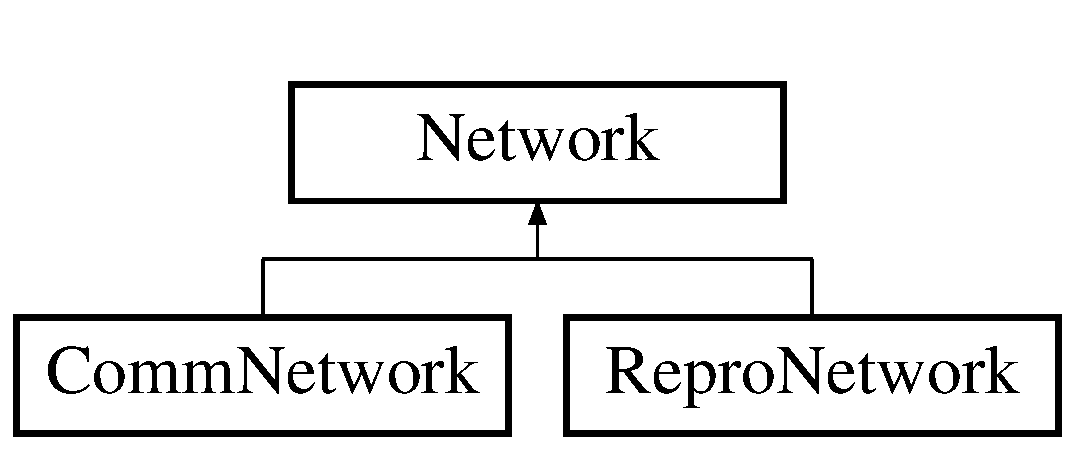
\includegraphics[height=2.000000cm]{class_network}
\end{center}
\end{figure}
\subsection*{Public Member Functions}
\begin{DoxyCompactItemize}
\item 
void \mbox{\hyperlink{class_network_a8285772739069a17a6cf3407208c25cb}{feed\+Forward}} ()
\begin{DoxyCompactList}\small\item\em Calls update value on each node in each layer \end{DoxyCompactList}\item 
\mbox{\hyperlink{class_network}{Network}} \mbox{\hyperlink{class_network_a08970b95e111e12a0463719c959db247}{get\+Shallow\+Copy}} ()
\end{DoxyCompactItemize}
\subsection*{Public Attributes}
\begin{DoxyCompactItemize}
\item 
List$<$ List$<$ \mbox{\hyperlink{class_node}{Node}} $>$ $>$ \mbox{\hyperlink{class_network_a5575fb3cc8b86da6ff8ffed15634e4b4}{net}} = new List$<$List$<$\mbox{\hyperlink{class_node}{Node}}$>$$>$()
\item 
string \mbox{\hyperlink{class_network_a9d47011c0cdd1c2c2a17f487fc20aa74}{name}}
\item 
int \mbox{\hyperlink{class_network_a28e1ac9d80508cd8bb52624e4e1efede}{in\+Layer}}
\end{DoxyCompactItemize}


\subsection{Detailed Description}
A neural network of a creature, which consists of layers of nodes. 



\subsection{Member Function Documentation}
\mbox{\Hypertarget{class_network_a8285772739069a17a6cf3407208c25cb}\label{class_network_a8285772739069a17a6cf3407208c25cb}} 
\index{Network@{Network}!feed\+Forward@{feed\+Forward}}
\index{feed\+Forward@{feed\+Forward}!Network@{Network}}
\subsubsection{\texorpdfstring{feed\+Forward()}{feedForward()}}
{\footnotesize\ttfamily void Network.\+feed\+Forward (\begin{DoxyParamCaption}{ }\end{DoxyParamCaption})}



Calls update value on each node in each layer 

\mbox{\Hypertarget{class_network_a08970b95e111e12a0463719c959db247}\label{class_network_a08970b95e111e12a0463719c959db247}} 
\index{Network@{Network}!get\+Shallow\+Copy@{get\+Shallow\+Copy}}
\index{get\+Shallow\+Copy@{get\+Shallow\+Copy}!Network@{Network}}
\subsubsection{\texorpdfstring{get\+Shallow\+Copy()}{getShallowCopy()}}
{\footnotesize\ttfamily \mbox{\hyperlink{class_network}{Network}} Network.\+get\+Shallow\+Copy (\begin{DoxyParamCaption}{ }\end{DoxyParamCaption})}



\subsection{Member Data Documentation}
\mbox{\Hypertarget{class_network_a28e1ac9d80508cd8bb52624e4e1efede}\label{class_network_a28e1ac9d80508cd8bb52624e4e1efede}} 
\index{Network@{Network}!in\+Layer@{in\+Layer}}
\index{in\+Layer@{in\+Layer}!Network@{Network}}
\subsubsection{\texorpdfstring{in\+Layer}{inLayer}}
{\footnotesize\ttfamily int Network.\+in\+Layer}

\mbox{\Hypertarget{class_network_a9d47011c0cdd1c2c2a17f487fc20aa74}\label{class_network_a9d47011c0cdd1c2c2a17f487fc20aa74}} 
\index{Network@{Network}!name@{name}}
\index{name@{name}!Network@{Network}}
\subsubsection{\texorpdfstring{name}{name}}
{\footnotesize\ttfamily string Network.\+name}

\mbox{\Hypertarget{class_network_a5575fb3cc8b86da6ff8ffed15634e4b4}\label{class_network_a5575fb3cc8b86da6ff8ffed15634e4b4}} 
\index{Network@{Network}!net@{net}}
\index{net@{net}!Network@{Network}}
\subsubsection{\texorpdfstring{net}{net}}
{\footnotesize\ttfamily List$<$List$<$\mbox{\hyperlink{class_node}{Node}}$>$ $>$ Network.\+net = new List$<$List$<$\mbox{\hyperlink{class_node}{Node}}$>$$>$()}



The documentation for this class was generated from the following file\+:\begin{DoxyCompactItemize}
\item 
\mbox{\hyperlink{_network_8cs}{Network.\+cs}}\end{DoxyCompactItemize}

\hypertarget{class_node}{}\section{Node Class Reference}
\label{class_node}\index{Node@{Node}}
\subsection*{Public Member Functions}
\begin{DoxyCompactItemize}
\item 
void \mbox{\hyperlink{class_node_a6700b2928da6ac5fcac8431d6f16597e}{append\+Input\+Node}} (\mbox{\hyperlink{class_node}{Node}} new\+Node)
\begin{DoxyCompactList}\small\item\em Adds a node to the array of input nodes. \end{DoxyCompactList}\item 
bool \mbox{\hyperlink{class_node_ae35ca95be4806e6a3f81617d888f724f}{remove\+Node}} (int remove\+Index)
\begin{DoxyCompactList}\small\item\em Remove node from input nodes. \end{DoxyCompactList}\end{DoxyCompactItemize}
\subsection*{Properties}
\begin{DoxyCompactItemize}
\item 
float \mbox{\hyperlink{class_node_a4d82b89fd1d72cc0184763279a3811dc}{value}}\hspace{0.3cm}{\ttfamily  \mbox{[}get, set\mbox{]}}
\begin{DoxyCompactList}\small\item\em The value of the node takes on based on it\textquotesingle{}s inputs and activation function. \end{DoxyCompactList}\end{DoxyCompactItemize}


\subsection{Member Function Documentation}
\mbox{\Hypertarget{class_node_a6700b2928da6ac5fcac8431d6f16597e}\label{class_node_a6700b2928da6ac5fcac8431d6f16597e}} 
\index{Node@{Node}!append\+Input\+Node@{append\+Input\+Node}}
\index{append\+Input\+Node@{append\+Input\+Node}!Node@{Node}}
\subsubsection{\texorpdfstring{append\+Input\+Node()}{appendInputNode()}}
{\footnotesize\ttfamily void Node.\+append\+Input\+Node (\begin{DoxyParamCaption}\item[{\mbox{\hyperlink{class_node}{Node}}}]{new\+Node }\end{DoxyParamCaption})}



Adds a node to the array of input nodes. 

\mbox{\Hypertarget{class_node_ae35ca95be4806e6a3f81617d888f724f}\label{class_node_ae35ca95be4806e6a3f81617d888f724f}} 
\index{Node@{Node}!remove\+Node@{remove\+Node}}
\index{remove\+Node@{remove\+Node}!Node@{Node}}
\subsubsection{\texorpdfstring{remove\+Node()}{removeNode()}}
{\footnotesize\ttfamily bool Node.\+remove\+Node (\begin{DoxyParamCaption}\item[{int}]{remove\+Index }\end{DoxyParamCaption})}



Remove node from input nodes. 


\begin{DoxyParams}{Parameters}
{\em remove\+Index} & Index of node to remove.\\
\hline
\end{DoxyParams}


\subsection{Property Documentation}
\mbox{\Hypertarget{class_node_a4d82b89fd1d72cc0184763279a3811dc}\label{class_node_a4d82b89fd1d72cc0184763279a3811dc}} 
\index{Node@{Node}!value@{value}}
\index{value@{value}!Node@{Node}}
\subsubsection{\texorpdfstring{value}{value}}
{\footnotesize\ttfamily float Node.\+value\hspace{0.3cm}{\ttfamily [get]}, {\ttfamily [set]}}



The value of the node takes on based on it\textquotesingle{}s inputs and activation function. 



The documentation for this class was generated from the following file\+:\begin{DoxyCompactItemize}
\item 
C\+:/\+Users/\+Brett/\+Documents/\+Git\+Hub/\+Unity/\+Eco\+Net/\+Assets/\+Scripts/Node.\+cs\end{DoxyCompactItemize}

%--- End generated contents ---

% Index
\backmatter
\newpage
\phantomsection
\clearemptydoublepage
\addcontentsline{toc}{chapter}{Index}
\printindex

\end{document}
